%Styles
\tikzstyle{ground}=[color=gray,postaction={draw,decorate,decoration={border,angle=-45,amplitude=0.2cm,segment length=2mm}}]
\tikzstyle{cart} = [draw, fill=cyan!10, rectangle, minimum height=1cm, minimum width=1.2cm, rounded corners =0.1cm,node distance=2cm]
\tikzstyle{actuator} = [draw=black ,fill=black!10!white, thick, rectangle, inner sep=0,minimum height=0.6cm, minimum width=0.2cm, node distance=3cm]
\tikzstyle{spring} = [thick,black,decorate,decoration={snake,amplitude=3,segment length=10}]
\tikzstyle{wheel} = [thick,orange,decorate,decoration={coil,aspect=0.7,amplitude=5}]
\tikzstyle{cart} = [rectangle, inner sep=0,minimum height=0.8cm, minimum width=1cm, node distance=3cm, path picture={ 
      \shadedraw[left color=white,right color=gray!40!white, thick] ([yshift=0.12cm, xshift=0.3pt] path picture bounding box.south west) rectangle ([xshift=-0.3pt,yshift=-0.3pt] path picture bounding box.north east); 
      \draw[very thick, fill=white] ([yshift=0.12cm, xshift=0.2cm] path picture bounding box.south west) circle (0.1cm);
      \draw[very thick,fill=white] ([yshift=0.12cm, xshift=-0.2cm] path picture bounding box.south east) circle (0.1cm);}]
\tikzstyle{pt} = [coordinate]
\tikzstyle{tf} = [draw,thick,shape=rectangle,inner sep=0,minimum height=0.7cm, minimum width=0.9cm]
\tikzstyle{math} = [draw, thick, circle, minimum size=0.6cm,node distance=2cm, path picture={ 
      \draw[] (path picture bounding box.south west) -- (path picture bounding box.north east);
      \draw[] (path picture bounding box.north west) -- (path picture bounding box.south east);}]
 
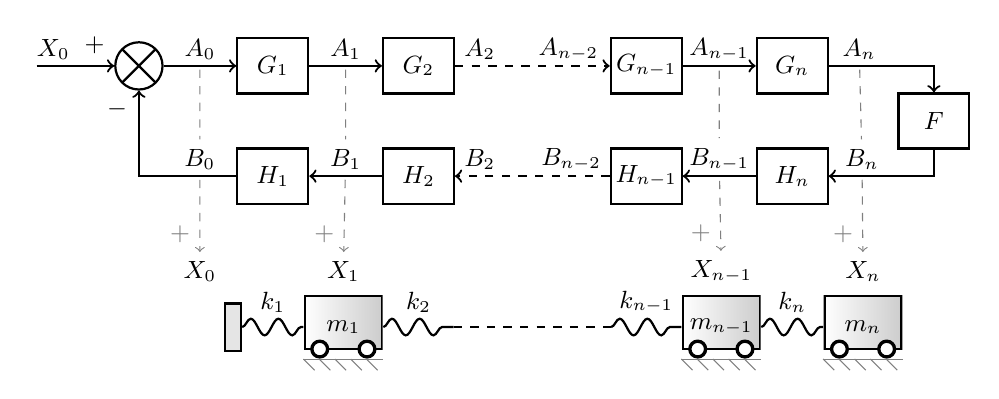
\begin{tikzpicture}[scale=1,every node/.style={font=\small}]


%Nodes

	\node[actuator]		(act) 				{};
	\node[cart]	(m1)		[right of=act, node distance=1.4cm]			{$m_1$};
       \node[pt] 	(pt1) 		[right of=m1, node distance=1.4cm] 	{};
	\node[pt] 	(pt2) 		[right of=pt1, node distance=2cm] 	{};
	\node[cart] 	(m3) 		[right of=pt2, node distance=1.4cm] 	{$m_{n-1}$};
	\node[cart] 	(m4) 		[right of=m3, node distance=1.8cm] 	{$m_n$};
%Connections	
	\draw[spring] (act) -- node[yshift=9pt] (k1){$k_1$} (m1);
	
	\draw[spring] (m1) -- node[yshift=9pt] (k2) {$k_2$} (pt1);
	\draw[thick, dashed] (pt1) -- (pt2);
	\draw[spring] (pt2) -- node[yshift=9pt] (k3) {$k_{n-1}$} (m3);
	\draw[spring] (m3) -- node[yshift=9pt] (k4) {$k_n$} (m4);
	
	\draw[ground] (m1.south west) -- (m1.south east);
	\draw[ground] (m4.south west) -- (m4.south east);
	\draw[ground] (m3.south west) -- (m3.south east);
	
	\node	(X0)		[above of=act, node distance = 20pt,xshift = -12pt]		{$X_0$};
	\node	(X1)		[above of=m1, node distance = 20pt]		{$X_1$};
	\node	(X2)		[above of=m3, node distance = 20pt]		{$X_{n-1}$};
	\node	(X3)		[above of=m4, node distance = 20pt]		{$X_n$};

       \node[tf]	(G1)		[below of=k1, node distance = -3cm]			{$G_1$};
	\node[tf]	(G2)		[below of=k2, node distance = -3cm]		{$G_2$};
	\node[tf]	(G3)		[below of=k3, node distance = -3cm]			{$G_{n-1}$};
	\node[tf]	(G4)		[below of=k4, node distance = -3cm]		{$G_n$};
	\node[tf]	(F)		[right of=G4, yshift=-0.7cm, node distance = 1.8cm]	{$F$};
	 \node[tf]	(H1)		[below of=G1, node distance = 1.4cm]			{$H_1$};
	\node[tf]	(H2)		[below of=G2, node distance = 1.4cm]		{$H_2$};
	\node[tf]	(H3)		[below of=G3, node distance = 1.4cm]			{$H_{n-1}$};
	\node[tf]	(H4)		[below of=G4, node distance = 1.4cm]		{$H_n$};

	\node[math]	(add)		[left of=G1, node distance = 1.7cm]	[label=175:$+$,label=265:$-$ ]			{};
	\node[pt]		(in)			[left of=add, node distance = 1.3cm]		{};
	       
	\draw[->,thick] (in)			-- node[xshift=-8pt, yshift=6pt] 			{ $X_0$} (add);	
       \draw[->,thick] (add) 		-- node[yshift=6pt] (A0) 					{ $A_0$} (G1);	
	\draw[->,thick] (G1)   		-- node[yshift=6pt] (A1)					{ $A_1$} (G2);
	\draw[->,thick,dashed] (G2) 	-- node[xshift=-19pt,yshift=6pt] (A2)	 	{$A_2$} node[xshift=13pt,yshift=6pt] (A3) {$A_{n-2}$} (G3);
	\draw[->,thick] (G3) 			-- node[yshift=6pt]	 		      (A4)		{ $A_{n-1}$} (G4);
	\draw[->,thick] (G4) 			-| node[xshift = -27pt,yshift=6pt]   (A5)	{ $A_n$} (F);
	\draw[->,thick] (F) 			|- node[xshift=-26pt, yshift=6pt] 	(B5)		{ $B_n$}(H4);
	\draw[->,thick] (H4) 		-- node[xshift=0pt, yshift=6pt] 		(B4)	{ $B_{n-1}$}(H3);
	\draw[->,thick,dashed] (H3) 	-- node[xshift=-19pt, yshift=6pt] (B2) 	{ $B_2$}  node[xshift=14pt, yshift=6pt] (B3) { $B_{n-2}$}  (H2);
	\draw[->,thick] (H2) 		-- node[xshift=0pt, yshift=6pt] 		(B1)	{ $B_1$} (H1);
	\draw[->,thick] (H1) 		-| node[xshift=22pt, yshift=6pt] 		(B0)	{ $B_0$} (add);
	
	\draw[->,dashed,gray] (A0) -- (B0) --node[near end, left] {$+$} (X0);
	\draw[->,dashed,gray] (A1) -- (B1) --node[near end, left] {$+$} (X1);
	\draw[->,dashed,gray] (A4) -- (B4) --node[near end, left] {$+$} (X2);
	\draw[->,dashed,gray] (A5) -- (B5) --node[near end, left] {$+$} (X3);
\end{tikzpicture}